% chapter 3 : teach center
\chapter{Teach Center}

Auf der offiziellen Seite des Teach Centers bietet die TU Graz einige Tutorials 
an:\linebreak\url{\tctugraz}\linebreak Viele der Möglichkeiten des TCs
werden im Rahmen der Lehrveranstaltung aber nicht benötigt (z.B. Foren,
Umfragen, etc.), weshalb hier die wirklich gebrauchten Funktionen nochmals
skizziert werden.

Das TC funktioniert grundsätzlich recht intuitiv. Man loggt sich ganz normal 
ein, hat aber mehr Rechte als der reguläre Studierende. Zuerst wird auf die
allgemeine Handhabung des TC eingegangen und dann die wichtigsten Funktionen 
der vier Reiter \twrite{Schwarzes Brett}, \twrite{Administratives}, 
\twrite{Unterlagen} und \twrite{Lehr- und Lernhilfen} beschrieben.

{\bf Wichtig:} Jedes Fach im TUGonline hat eine eigene Teach Center Gruppe. 
Es gibt eine eige Gruppen für {\tt Mechanik B3}, 
{\tt Dynamik VT}, {\tt Mechanik - Dynamik (VO)} und 
{\tt Mechanik - Dynamik (UE)}. Wird also eine Verlautbarung auf das Schwarze
Brett von {\tt Dynamik VT} gestellt, so muss sie für alle anderen Gruppen
kopiert werden. Analog verhält es sich mit den Unterlagen: Skriptum und
Übungsblätter müssen in alle TC-Gruppen separat hochgeladen werden (natürlich
müssen übungszogene Inhalte nicht in die {\tt Mechanik - Dynamik (UE)}
gestellt werden). Die einzige Ausnahme hierbei ist die Anmeldung zur
Übungsblattabgabe, welche nur ein einiziges mal in der Gruppe 
{\tt Baumechanik 3 (Mechanik B3)} erstellt werden muss. Damit aber alle
Studierenden wissen, wo sie sich anzumelden haben, muss in den anderen Gruppen
die Anmeldung verlinkt werden. Wie man hier vorgeht wird noch im Part zur
Anmeldung zur Übungsblattabgabe detailliert.

\section{Allgemeine Funktionen}

Die allgemeinen Funktionen finden sich, wie in \figref{fig:general} dargestellt,
rechts oben, wobei die einzig wichtigeen Punkt \twrite{Administration} und
\twrite{Benutzer} sind.

\begin{figure}[htbp]
\begin{center}
  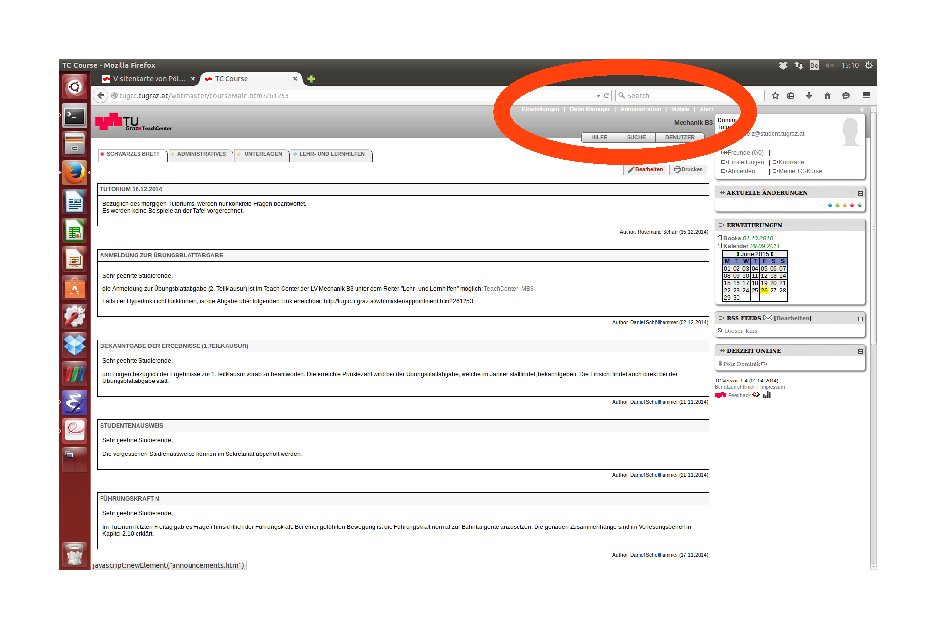
\includegraphics[width=.75\textwidth]{3_general.pdf}
  \caption{ Die allgemeinen Funktionen. In der ersten Zeile ist nur 
    \twrite{Administration} und in der zweiten nur \twrite{Benutzer} relevant.}
  \label{fig:general}
\end{center}
\end{figure}

Im Folgenden gehen wir auf die wichtigsten Funktionen von
\twrite{Administration} ein.

\subsection{Administration - Parameter}

Hier können neue \glqq{}Course Tutors\grqq{}, also Studienassistenten mit
Schreibrechten in der TC Gruppe, hinzugefügt werden. Um dies zu tun, muss in
der Zeile \twrite{Course Tutors} - dargestellt in \figref{fig:params} - 
die TUG-ID des Nutzers hinzugefügt werden, wobei die einzelnen IDs durch ein 
Semikolon getrennt sind. Danach muss die neue Liste unten mit dem Button 
\twrite{Ok} bestätigt werden. Natürlich können auch bestehende Zugriffsrechte 
durch Entfernen der Nutzer-IDs entzogen werden. Alle weiteren Funktionen werden 
praktisch nicht benötigt.

{\bf Herausfinden der TUG-ID:} Loggt man sich ins TC mit seinem Account ein, so
sieht man auf der rechten Seite die Kurskarte und ganz rechts oben seinen Namen.
Man klickt auf diesen und im folgenden Fenster klickt man auf
\twrite{Bearbeiten}. Es öffnet sich ein Fenster, und in der ersten Zeile
steht {\tt Modify Account \grqq{}<ID>\grqq{}}, wobei {\tt <ID>} die gesuchte
ID ist.

\begin{figure}[htbp]
\begin{center}
  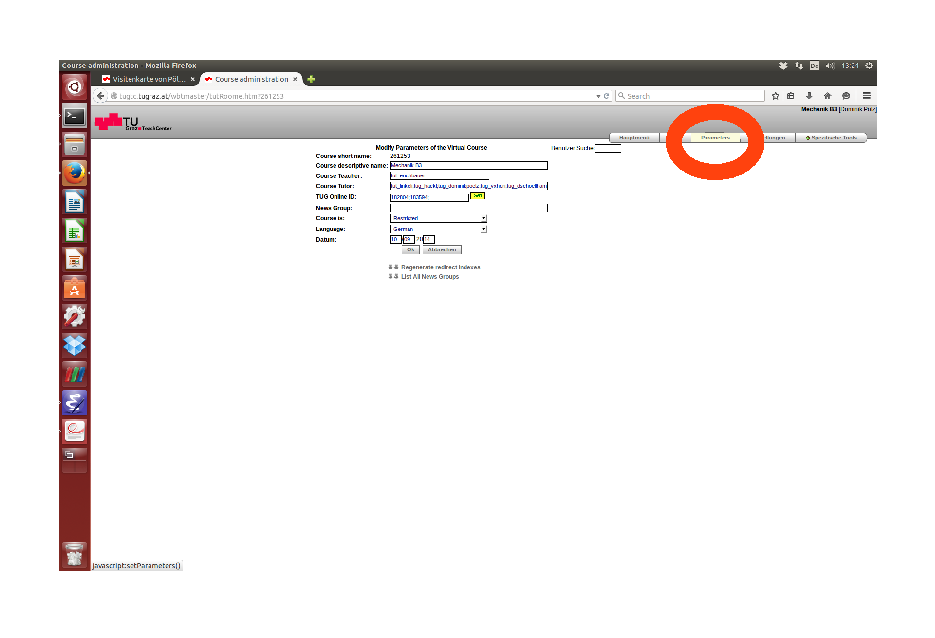
\includegraphics[width=\textwidth]{3_params.pdf}
  \caption{ \twrite{Administration} - \twrite{Parameters} }
  \label{fig:params}
\end{center}
\end{figure}

\subsection{Administration - Einstellungen}

Hier können Funktionen des TC ein- und ausgeschaltet werden, wie beispielsweise
das Forum. Im Allgemeinen müssen aber keine Änderungen vorgenommen werden.

\subsection{Benutzer}

Hier werden die Leserechte an der TC Gruppe geregelt, d.h. alle hier 
eingetragenen Studierende haben Zugriff zur Gruppe. 

\subsubsection{Exportierung Teilnehmerliste}

Um eine Teilnehmerliste aus dem Teach Center in Excel zu exportieren müssen
folgende Schritte unternommen werden (\figref{fig:export} stellt diesen
Prozess grafisch dar):

\begin{enumerate}
\item Button \twrite{Benutzer}
\item Button \twrite{Liste drucken}
\item Button \twrite{Alle auswählen}
\item Button \twrite{Exportieren} und Button \twrite{CSV exportieren}
\item Im Fenster {\bf ctrl-a} (alles auswählen) und {\bf ctrl-c} (kopieren)
  drücken.
\item Im Excel {\bf ctrl-v} (einfügen) drücken. Darauf folgt ein Dialog zur
  Importierung: Hier muss als Trennsymbol (\glqq{}separator symbol\grqq{})
  der Semikolon gewählt werden. In der unteren Vorschau kann man dann erkennen,
  das die Daten in drei Spalten getrennt werden.
\end{enumerate}

\begin{figure}[htbp]
  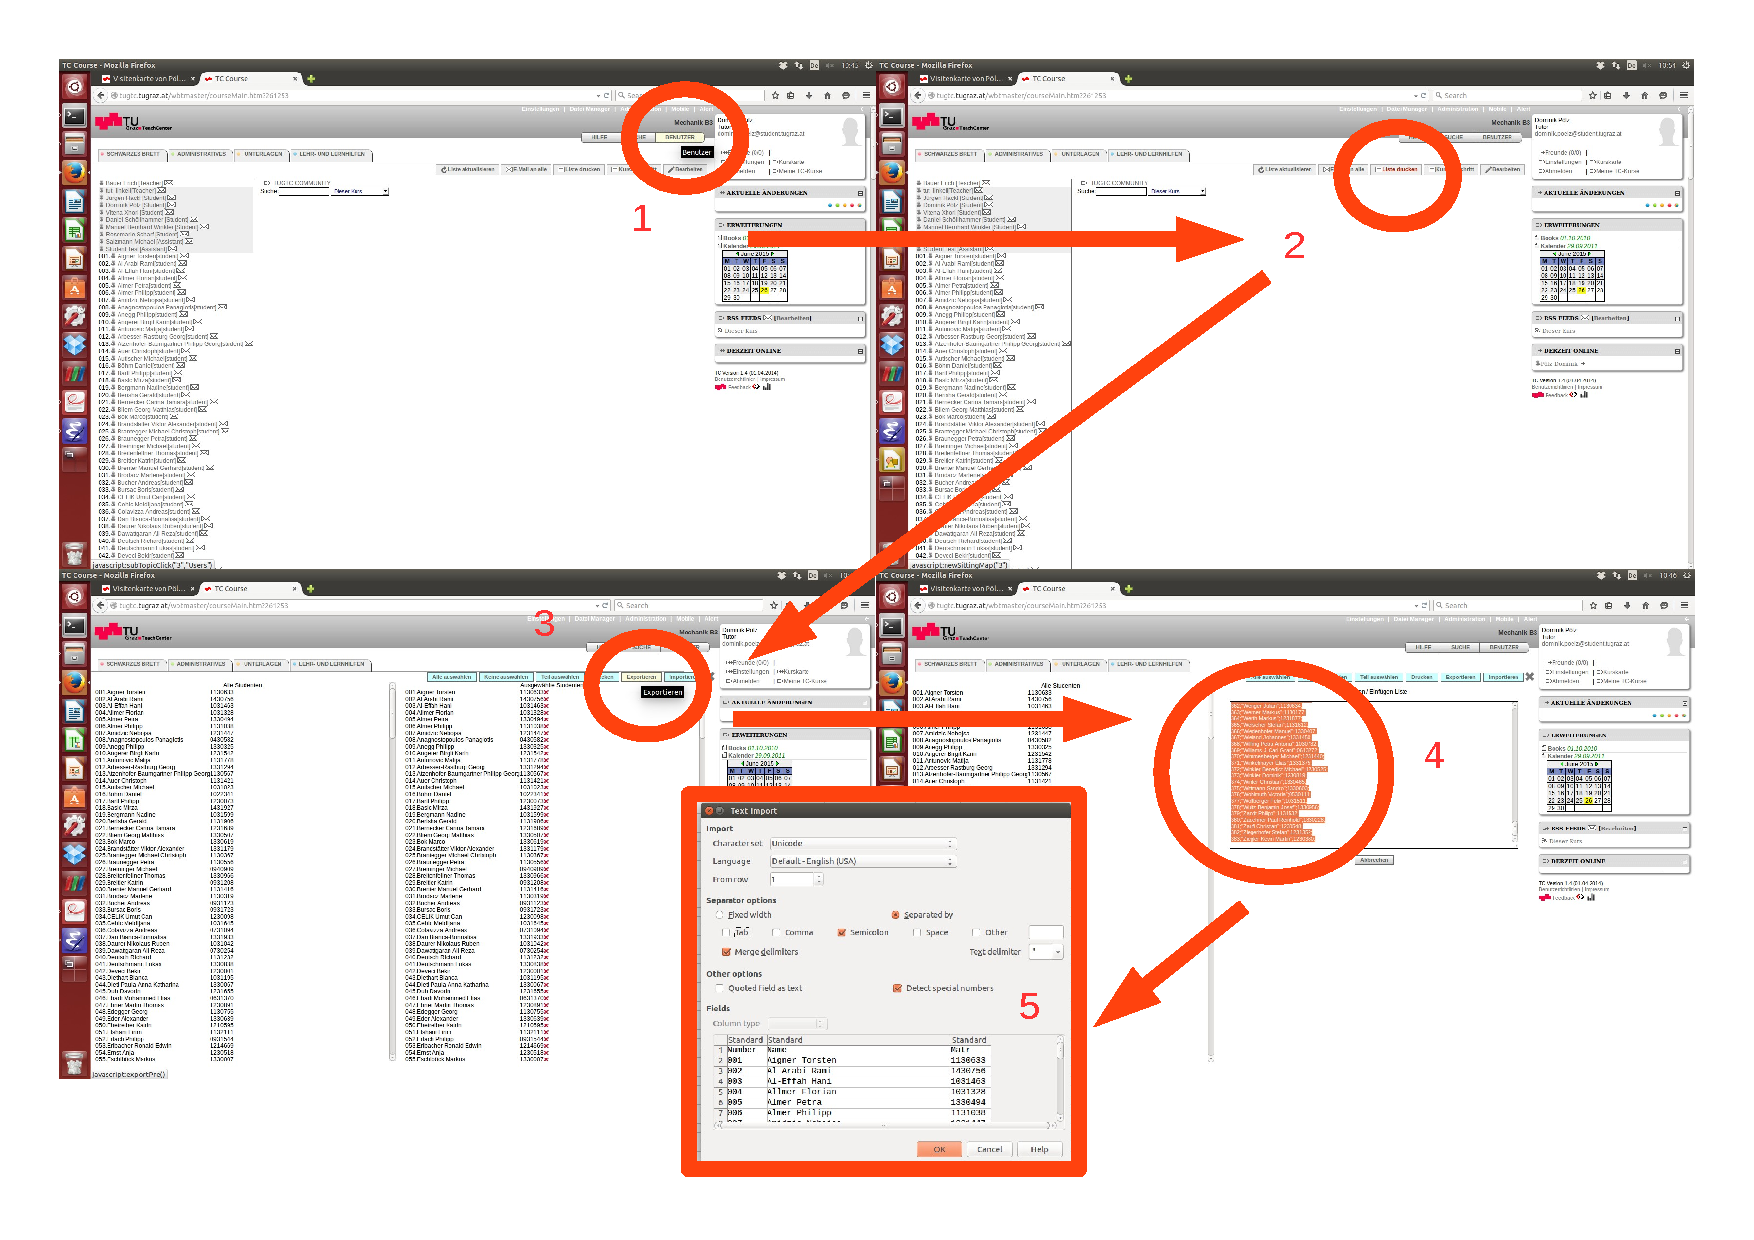
\includegraphics[width=\textwidth]{3_exportList.pdf}
  \caption{ (1) Auswahl Benutzer. (2) Liste drucken. (3) Alle ausw\"{a}hlen und
    exportieren. (4) Gesamten Inhalt kopieren und (5) in Excel einf\"{u}gen,
    wobei das richtige Trennsymbol zu w\"{a}hlen ist.}
  \label{fig:export}
\end{figure}

\subsubsection{Hinzufügen von Studierenden}

Manchmal kommt es vor, dass einzelne Studierende zur Lehrveranstaltung
nachgemeldet werden. Diese haben standardmäßig keine Zugriffsrechte auf das
TC, und müssen somit manuell hinzugefügt werden.

Wichtig ist hierbei Folgendes: Das 
\glqq{}Hinzufügen von Studierenden ins TC\grqq{} ist Nichts anderes, als eine 
Synchronisierung der Liste von Studenten die im TUGonline zur Lehrveranstaltung 
angemeldet sind, d.h. man muss nicht einzelne Studierende per Hand einfügen, 
sondern führt einfach einen {\bf refresh} der Liste aus.

Um die Liste zu aktualisieren, muss folgendes gemacht werden.
\begin{enumerate}
\item Button \twrite{Benutzer}
\item Button \twrite{Bearbeiten}
\item Button \twrite{Import}, siehe \figref{fig:import}
\end{enumerate}

Folgendes ist essentiell: Dieser Prozess kopiert die aktuelle Liste der zur
Lehrveranstaltung gemeldeten Studierenden des TUGonline und überschreibt die
TC-Liste. Um einen Studierenden also wirklich hinzufügen zu können, muss er zur
Lehveranstaltung gemeldet sein. Studienassistenten haben aber keine Rechte, um
Studierende im TUGonline nachzumelden, und somit muss der Studierende zuerst
vom Sekretariat im TUGonline  nachgemeldet werden, bevor man ihn/sie ins TC
importieren kann.

\begin{figure}[htbp]
  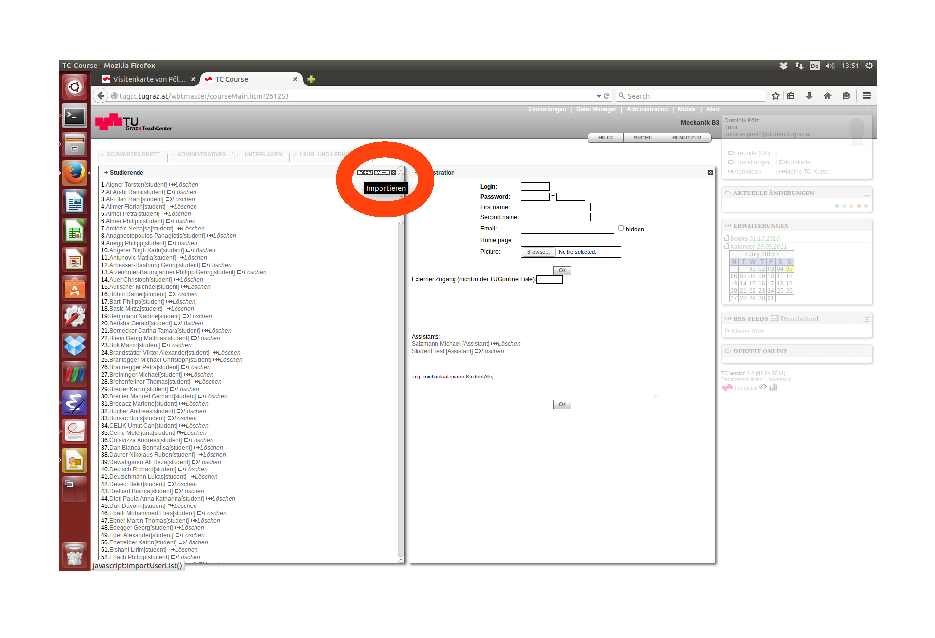
\includegraphics[width=\textwidth]{3_import.pdf}
  \caption{ Import der Liste der Studierenden.}
  \label{fig:import}
\end{figure}

\section{Schwarzes Brett}

Hier werden aktuelle Informationen bzw. Ankündigungen hineingeschrieben. Um
einen neuen Beitrag zu erstellen bzw. einen bestehenden zu editieren, muss
folgendes gemacht werden (siehe dazu \figref{fig:sb}):
\begin{enumerate}
\item Button \twrite{Bearbeiten}
\item Button \twrite{Neu} oder \twrite{Edit}
\end{enumerate}

Daraufhin öffnet sich ein Editor, in dem man den Text schreiben kann. Durch
Klick auf \twrite{HTML Editor} wechselt man auf einen WYSIWYG\footnotemark[1]
-Editor, in dem die HTML-tags automatisch erzeugt werden (wenn man den Text
fertig geschrieben hat, kann man ihn unten mit \twrite{Submit} in den
normalen Editor überspielen). Unten gibt es noch ein paar weitere Optionen,
die man aber meist nicht braucht.

\footnotetext[1]{\glqq{}what you see is what you get\grqq{} - Man sieht das
fertige Ergebnis und keine Kommandos. Auf dem Montitor erscheint nicht
\twrite{<strong>Text</strong>} sondern {\bf Text}.}

\begin{figure}[htbp]
  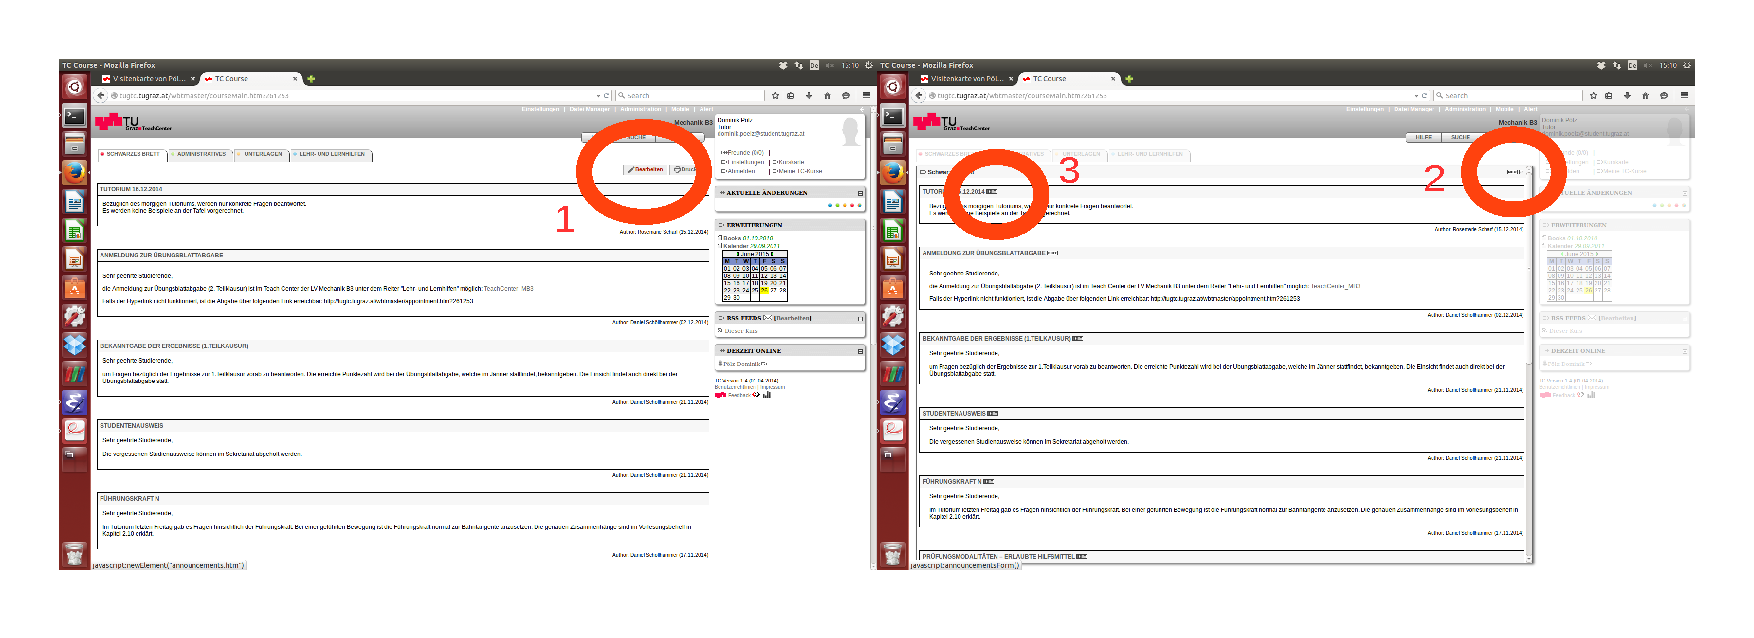
\includegraphics[width=\textwidth]{3_sb.pdf}
  \caption{ (1) Editieren des Schwarzen Brettes. (2) Erstellen eines neuen
    Beitrags. (3) Editieren eines bestehenden Beitrags.}
  \label{fig:sb}
\end{figure}

\section{Administratives}

Hier müssen die {\tt .pdf}-Files des Studenplans und der Prüfungsmodalitäten
hochgeladen werden. Der Prozess ist ähnlich wie beim \twrite{Schwarzen Brett}:
\begin{enumerate}
\item Button \twrite{Bearbeiten}
\item Eingabe von Titel und Text
\item Button \twrite{File hochladen} (unten) um die {\tt .pdf}-Files hochzuladen
\end{enumerate}


\section{Unterlagen}

Hier sind die {\tt .pdf}-Dateien des Vorlesungsbehelfs und der Angabe der
Übungsblätter hochzuladen. Dies funktioniert im Endeffekt gleich wie bei
\twrite{Administratives}
\begin{enumerate}
\item Button \twrite{Bearbeiten}
\item Links: \twrite{Neues File} $\to$ \twrite{Browse}, Datei auswählen
  $\to$ \twrite{Ok}
\item Rechts: Mit \twrite{Bearbeiten} bestehende Files editieren/löschen
\end{enumerate}


\section{Lehr- und Lernhilfen}

Hier müssen einerseits die {\tt .pdf}-Files des Durchgerechneten Beispiele und
der Lösungen hochgeladen werde, und andererseits die Anmeldung zur 
Übungsblattabgabe erstellt werden. Ersteres funktioniert genau wie bei
\twrite{Unterlagen}.

Grundsätzlich sollte die Gruppeneinteilung vom Vorjahr noch vorhanden sein, und
nicht gelöscht werden. Wurde sie aber gelöscht, so wird eine neue wie folgt
erstellt:
\begin{enumerate}
\item Button \twrite{Bearbeiten}
\item Links: \twrite{Add TC Components} $\to$ \twrite{Kursspezifische Tools}
  $\to$ \twrite{Online-Einteilung}
\end{enumerate}

{\bf Wichtig:}
Wie bereits zu Beginn dieses Kapitels angemerkt, muss diese Anmeldung nur in
der Gruppe {\tt Mechanik B3} erstellt werden, da alle anderen Studierenden
darauf Zugriff haben. Um es einfacher zu gestalten, die Anmeldung
zu finden, sollte in den TC-Gruppe {\tt Dynamik VT} und 
{\tt Mechanik-Dynamik (UE)} ein kurzer Eintrag am Schwarzen Brett erstellt 
werden. In diesem sind die Studierenden darauf zu hinzuweisen, dass die 
Anmeldung zur Übungsblattabgabe in Kürze beginnen wird/gerade begonnen hat und 
diese zu verlinken.

Der Link kann durch einen anchor so erstellt werden:\\
{\bf
<a href= \grqq{}LINK\grqq{}>TeachCenter\_MB3</a>
}

wobei \textbf{LINK} genau jene URL ist, die im Browser angezeigt wird, wenn
man in der Gruppen-Einteilung ist. Zum Vergleich lautete dieser Link
im Studienjahr 2014/15:\\
{\bf http://tugtc.tugraz.at/wbtmaster/appointment.htm?261253 }

Der Name zwischen {\bf <a>} und  {\bf </a>} kann natürlich beliebig
angepasst werden. Weiters ist es noch sinnvoll, den ganzen Link auch nochmal
in textlicher Form in den Eintrag am Schwarzen Brett zu inkludieren, zumal
der anchor bei einigen Browser nicht funktionieren könnte.


\subsection{Gruppen-Einteilung (Appointments)}

Die Gruppeneinteilung wird in \figref{fig:groups} dargestellt. Hierbei ist zu
beachten, dass die gesamte Abgabe eines Jahres ein einziges \twrite{Meeting}
ist, und die einzelnen Gruppen TC-intern als \twrite{Groups} bezeichnet werden.
Um sie zu editieren, muss rechts oben auf \twrite{Tools} geklickt werden, und
die einzelnen Aktionen werden im Folgenden noch genauer beschrieben.

\begin{figure}[htbp]
\begin{center}
  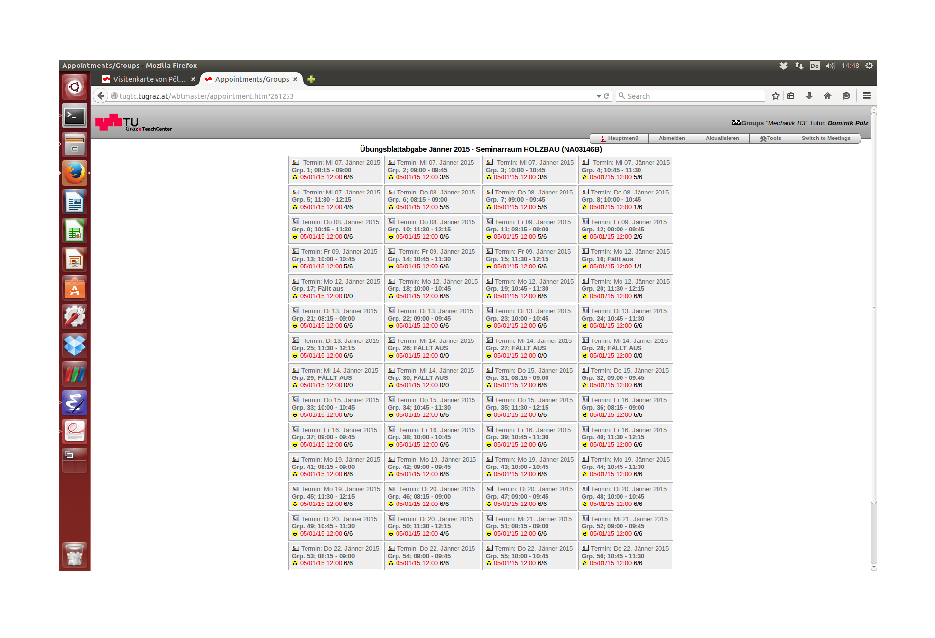
\includegraphics[width=.75\textwidth]{3_groups.pdf}
  \caption{ Gruppen-Einteilung.}
  \label{fig:groups}
\end{center}
\end{figure}

\subsubsection{Tools - Einstellungen}

Unter \twrite{Tools} $\to$ \twrite{Einstellungen} 
(dargestellt in \figref{fig:toolspref}) finden sich die wichtigsten Optionen zur
Übungsblattabgabe:
\begin{itemize}
\item \twrite{Meetings:} Übungsblattabgabe Jänner 20xx\\
  \twrite{Max. Appointments:} 1
\item \twrite{Groups:} Übungsblattabgabe Jänner 20xx - <Raum> (<Raumnummer>)\\
  \twrite{Group Max. Members:} 6
\item \twrite{Sperren/Free:}
  \begin{itemize}
    \item  Anmeldung ab gewissem Zeitpunkt erlauben: 
      \twrite{Sperren till-:} <Zeitpunkt>
    \item  Anmeldung bis zu gewissem Zeitpunkt erlauben: 
      \twrite{Free till-:} <Zeitpunkt>\\
      Muss nicht eingestellt werden, da die Anmeldung bis zu einem gewissen
      Zeitpunkt in den Gruppen erfolgt.
    \item <Zeitpunkt> im Format [yymmddhhmm]: 1501051200 ist beispielsweise
      der 5. Jänner 2015 um 12:00 Uhr.
  \end{itemize}
\end{itemize}

\begin{figure}[htbp]
  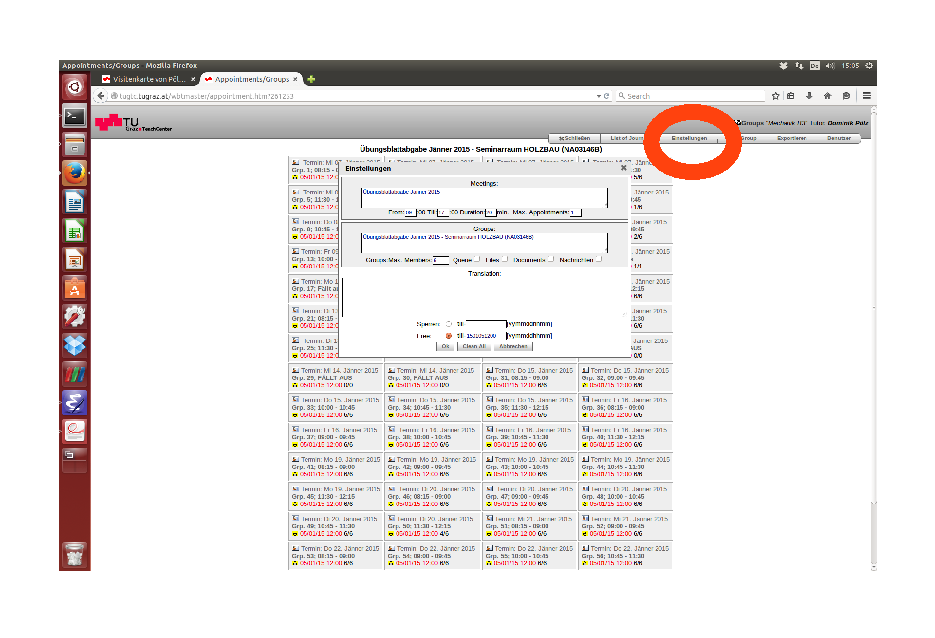
\includegraphics[width=\textwidth]{3_toolspref.pdf}
  \caption{ Tools - Einstellungen.}
  \label{fig:toolspref}
\end{figure}

\subsubsection{Tools - New Group}

Unter \twrite{Tools} $\to$ \twrite{New Group} 
(siehe \figref{fig:toolsnew}) können neue Gruppen erstellt werden:
\begin{itemize}
\item \twrite{Titel:} 
  Hier sollte folgender Vorlagentext hineingeschrieben werden:\\
  {\bf Termin: Mi 07. Jänner 2015<br><strong>Grp. 1; 08:15 - 09:00</strong>}\\
  Die einzelnen Zeiten und Gruppennummern müssen dann noch manuell eingetragen
  werden, aber die richtigen Kommandos für das Layout sind damit schon mal
  aufgesetzt (\twrite{<br>} sorgt für einen Zeilenumbruch und der Text
  zwischen \twrite{<strong>} und \twrite{<\textbackslash strong>} wird fett 
  gedruckt).
\item \twrite{Number of Groups:} xx\\
  So viele Gruppen wie benötigt. Dies ist beispielsweise aus dem Stundenplan 
  ersichtlich.
\item \twrite{Registration till-:}\\
  Hier wird der Endzeitpunkt der Anmeldung für alle Gruppen fixiert. (Der
  Beginnzeitpunkt wurde vorher bereits in den Einstellungen definiert).  
\end{itemize}

\begin{figure}[htbp]
  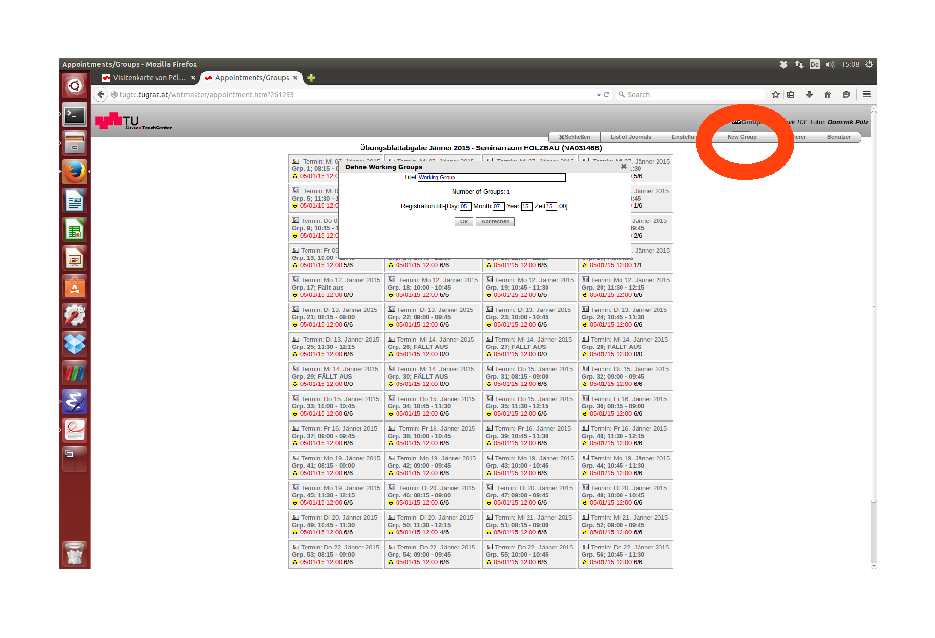
\includegraphics[width=\textwidth]{3_toolsnew.pdf}
  \caption{ Tools - New Group.}
  \label{fig:toolsnew}
\end{figure}

Somit werden alle Gruppen entsprechend der Vorlage erstellt. Nun muss noch jede
Gruppe per Hand mit Nummer und Zeit versehen werde, was im Folgenden beschrieben
wird.

\subsubsection{Gruppe editieren}

Um eine Gruppe zu bearbeiten klickt man in der Liste aller Gruppen den Titel
der gewünschten Gruppe, der nach der Vorlage 
\glqq{}Termin: Mi 07. Jänner 2015 {\bf Grp. 1; 08:15 - 09:00}\grqq{} lautet.
Darauf öffnet sich ein Fenster, in dem man durch Klick auf \twrite{Bearbeiten}
zu den einzelnen Eigenschaften der Gruppe gelangt (siehe 
\figref{fig:toolsgroup}). Hier muss in jeder Gruppe im Feld \twrite{Titel} das
Datum, die fortlaufende Gruppennummer und die Uhrzeit eingegeben werden.

Sollte ein Termin ausfallen, so kann hier z.B. die Uhrzeit durch 
\glqq{}ENTFÄLLT\grqq{} ersetzt werden und im Feld \twrite{Registration till-}
ein Termin in der Vergangenheit angegeben werden (somit existiert die Gruppe
noch, aber niemand kann sich anmelden).

\begin{figure}[htbp]
  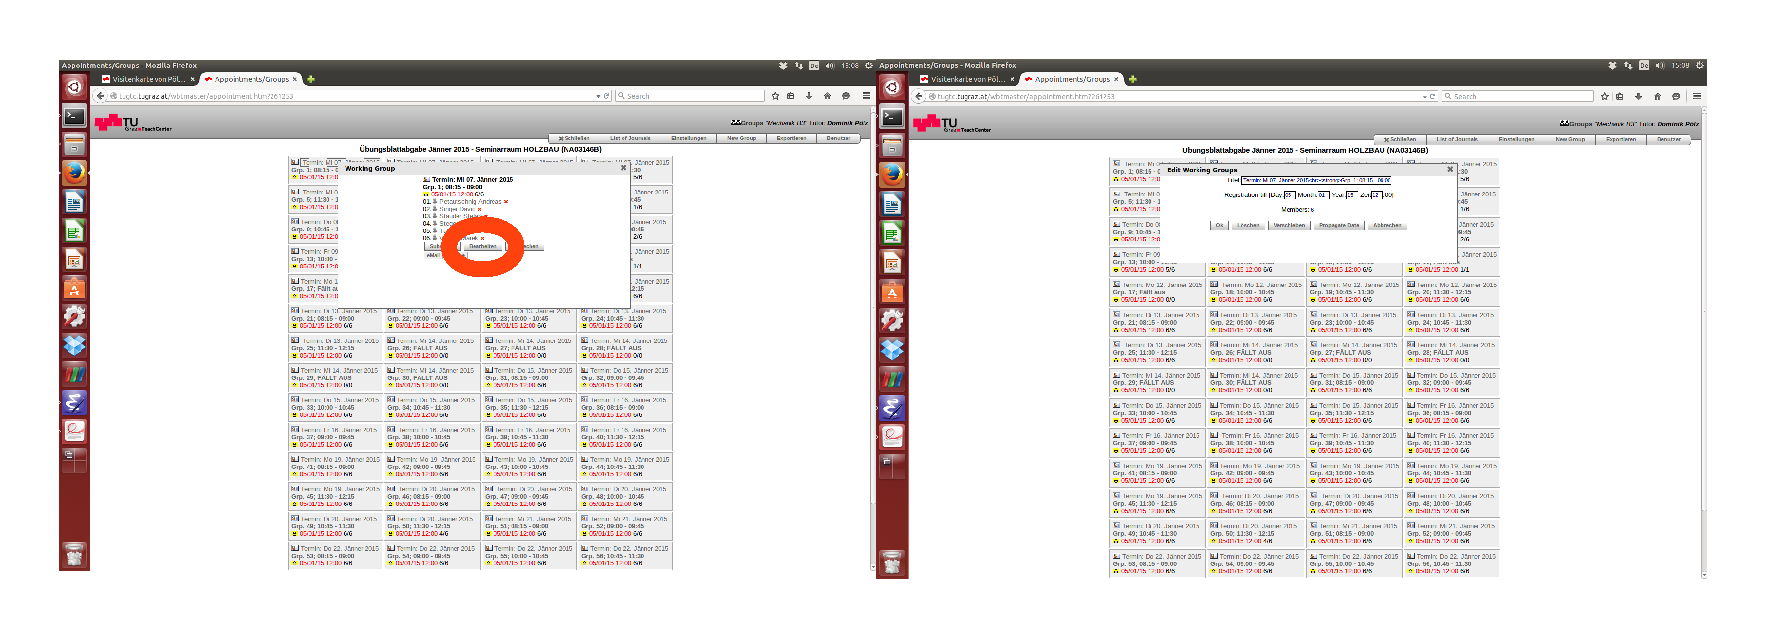
\includegraphics[width=\textwidth]{3_toolsgroup.pdf}
  \caption{ Bearbeiten der einzelnen Gruppen.}
  \label{fig:toolsgroup}
\end{figure}

\newpage
\subsubsection{Exportieren}

Nach Ende der Anmeldungsfrist, muss die Teilnehmerliste jeder Gruppe exportiert
werden. Dieser Prozess wird nun beschrieben:
\begin{enumerate}
  \item \twrite{Tools} $\to$ \twrite{Exportieren} 
  \item \twrite{All Groups} $\to$ \twrite{CSV} (siehe \figref{fig:exportall})
  \item Im Fenster \twrite{Copy/Paste} {\bf ctrl-a} (alles auswählen) und 
    {\bf ctrl-c} (kopieren) drücken (siehe \figref{fig:copypaste}).
 \item Den Inhalt in einen Texteditor (z.B. \twrite{notepad}, \twrite{notepad++}
    oder \twrite{emacs} kopieren.
 \item Alle HTML-tags entfernen:
    \begin{itemize}
      \item Ersetze: <br> durch \twrite{void}
      \item Ersetze: <strong> durch \twrite{void}
      \item Ersetze: </strong> durch \twrite{void}
      \item Ersetze: \grqq{} durch \twrite{void} \footnotemark[2]
      \item \twrite{void} bedeutet ein leeres Feld (kein Leerzeichen, sondern
        wirklich Nichts)
    \end{itemize}
  \item Den modifizierten Text mit {\bf ctrl-a} und {\bf ctrl-c} kopieren und
    dann mit {\bf ctrl-v} in Excel einfügen.
  \item Trennsymbol (\glqq{}separator symbol\grqq{}): Hier darf nur das
    Semikolon verwendet werden. Das Leerzeichen (Space) darf nicht verwendet
    werden, da sonst die Aufteilung der Spalten keinen Sinn ergibt.
\end{enumerate}

\footnotetext[2]{Das Zeichen \grqq{} erhählt man auf deutschen Keyboards durch 
{\bf shift-2}.}

Bei den eigentlichen Excel Dateien der Teilnehmerlisten sollte man sich sehr
stark an den Listen der Vorjahre orientieren, d.h. die Liste des vergangenen
Jahres kopieren und das sheet der {\tt csv} Datei mit der neuen Liste
überschreiben.

\begin{figure}[htbp]
\begin{center}
  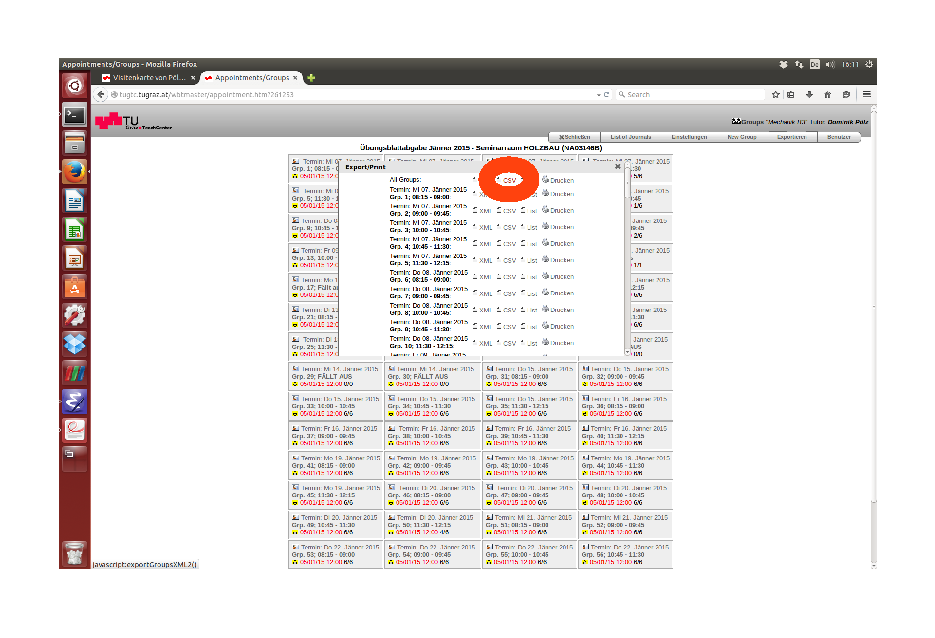
\includegraphics[width=.94\textwidth]{3_exportall.pdf}
  \caption{ Alle Gruppen als {\tt CSV} exportieren.}
  \label{fig:exportall}
\end{center}
\end{figure}

\begin{figure}[htbp]
\begin{center}
  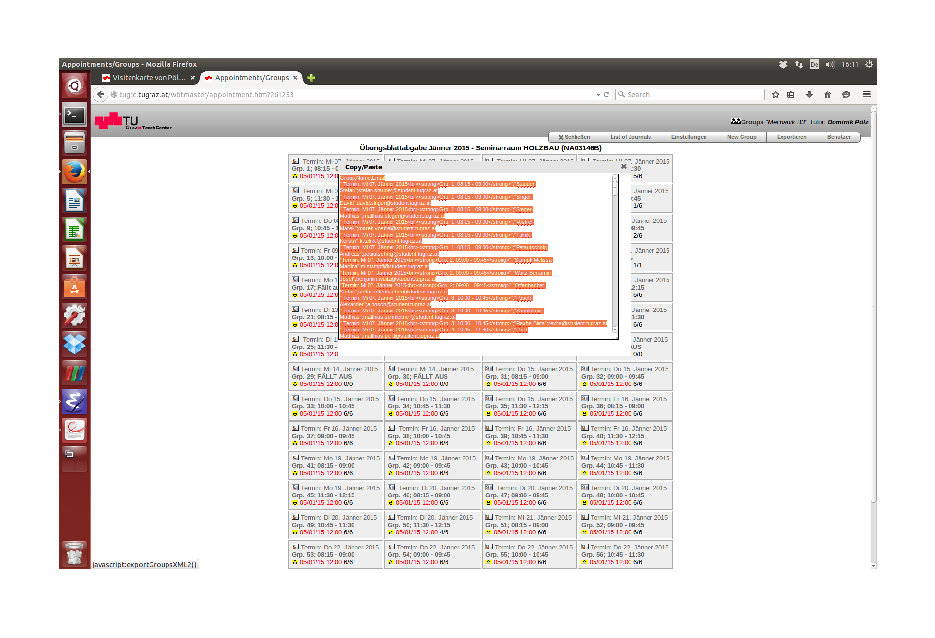
\includegraphics[width=.94\textwidth]{3_copypaste.pdf}
  \caption{ Copy/Paste.}
  \label{fig:copypaste}
\end{center}
\end{figure}

% EOF